\section{DFDs}
A data flow diagram (DFD) is a graphical representation of the "flow" of data through an information system, modeling its process aspects. A DFD is often used as a preliminary step to create an overview of the system, which can later be elaborated. DFDs of DoS is as following-:
\begin{enumerate}
\item Data flow LEVEL 0 figure \ref{fig:DFDs}
\item Data flow LEVEL 1 figure \ref{fig:DFDs1}
\end{enumerate}

\begin{figure}
\centering
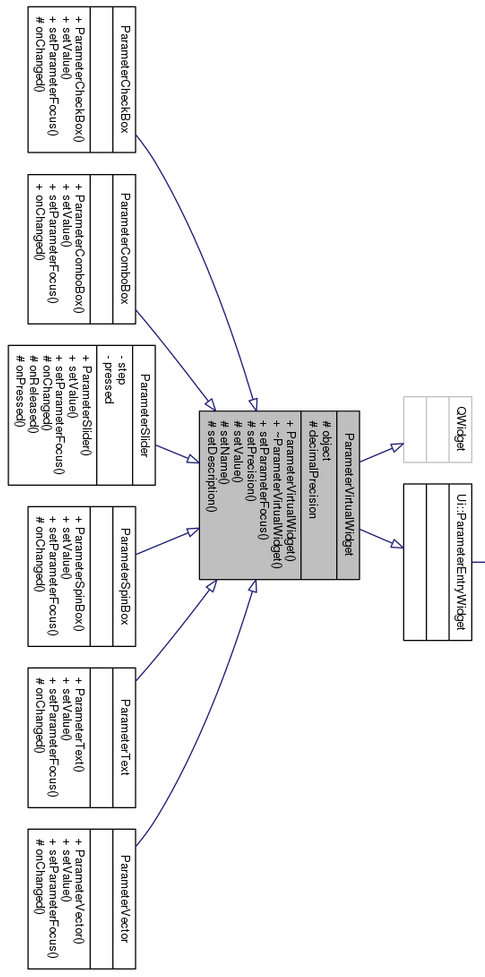
\includegraphics[width=0.7\linewidth]{images/collaborative1}
\caption{}
\label{fig:collaborative1}
\end{figure}
\begin{figure}
\centering

\includegraphics[width=0.7\linewidth]{images/comment}
\caption{}
\label{fig:comment}
\end{figure}
\begin{figure}
\centering
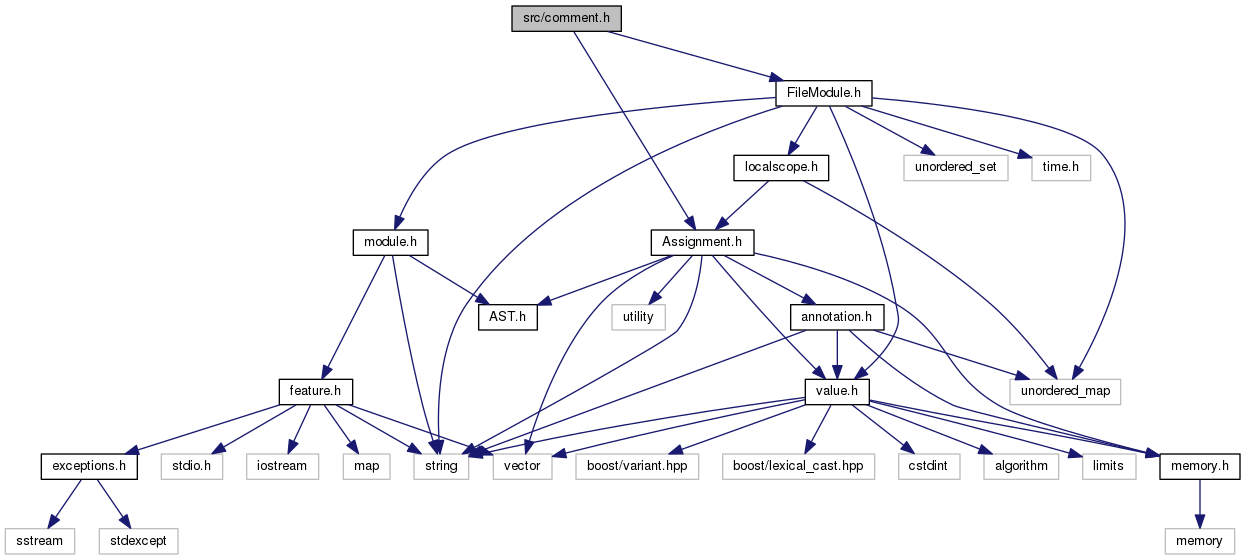
\includegraphics[width=0.7\linewidth]{images/comment1}
\caption{}
\label{fig:comment1}
\end{figure}

Here, In figure \ref{fig:DFDs} and figure \ref{fig:DFDs1}
\begin{enumerate}
\item MSG means Message
\item initial represent all initial input value
\item matrix represent all Mass, Height, Stiffness matrix
\end{enumerate}
\begin{figure}
\centering
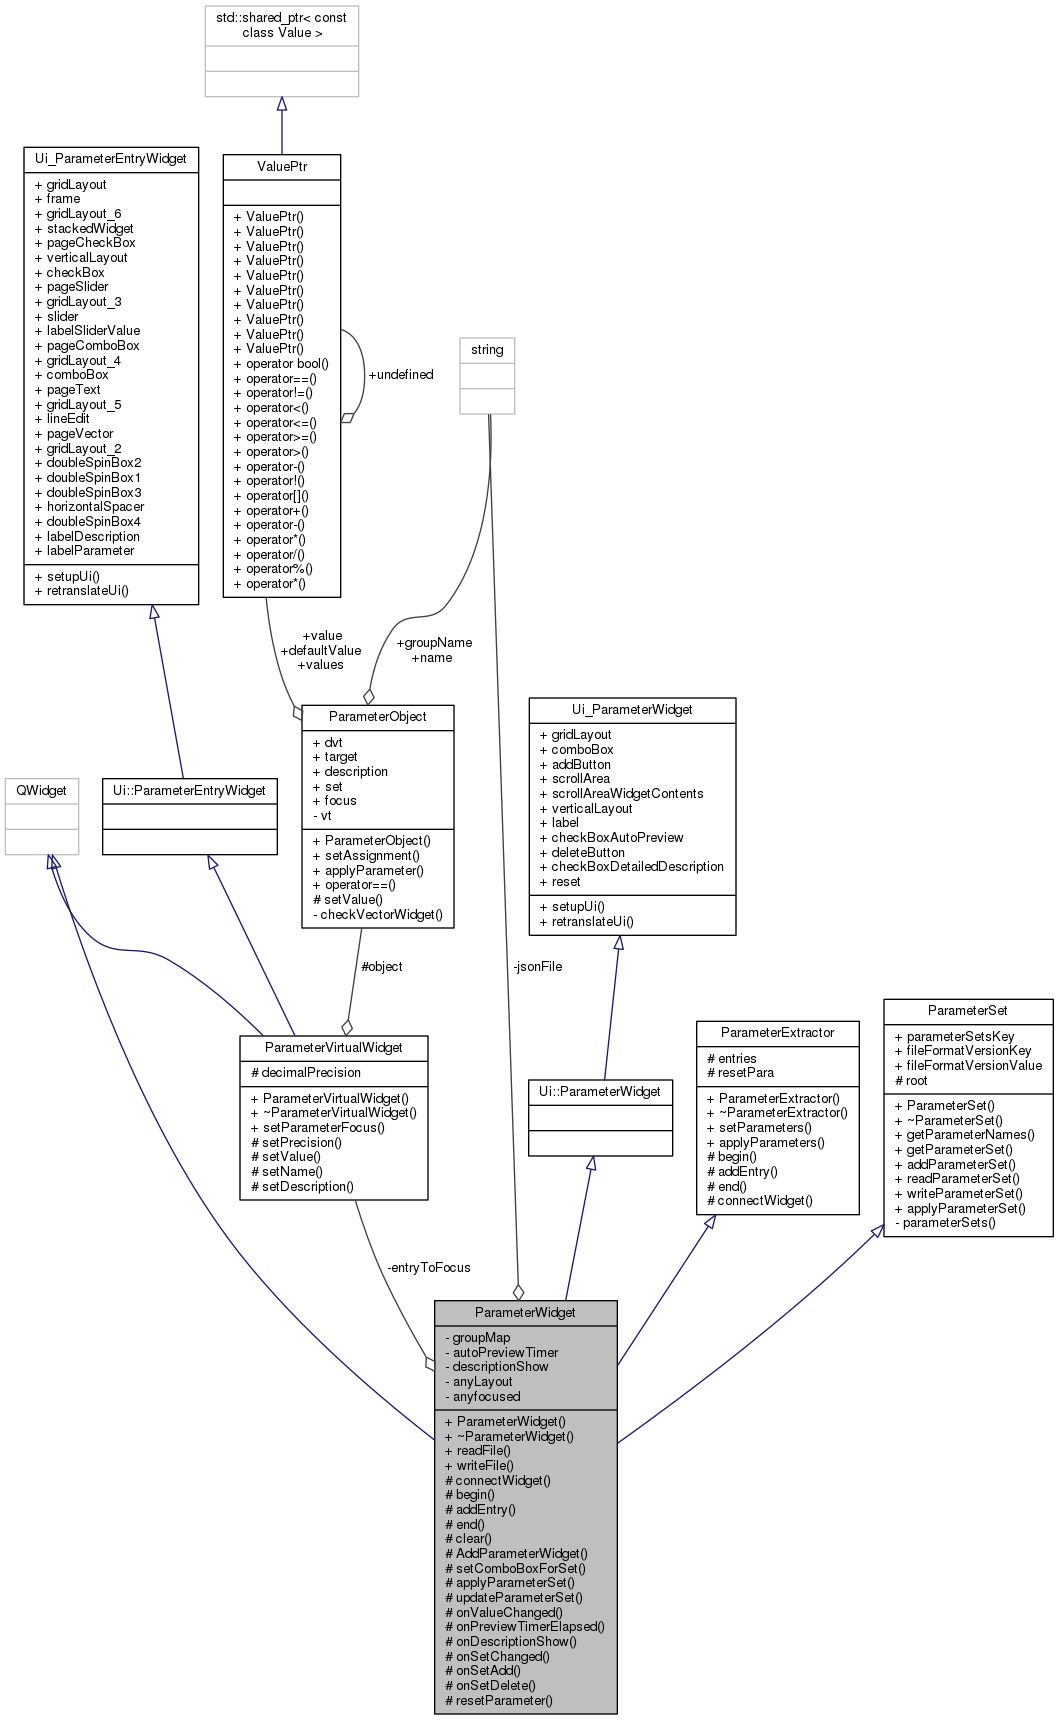
\includegraphics[scale=0.40]{images/collaborative}
\caption{Data Flow LEVEL 1}
\label{fig:collaborative}
\end{figure}

\section{Flowchart}
A flowchart is a type of diagram that represents an algorithm, work flow or process, showing the steps as boxes of various kinds, and their order by connecting them with arrows
and following are flowchart of DoS showing flow of control and Data in the software-:

Detailed Description[edit]

The basic implementation of the this project is almost done in form of prototype. There is need to modify structure of the project.We have to divide the task in to there parts:
Image05.png

Front end
It will deal with how the parameter will look to user like in form of range or spinbox etc. This part will include two parts:

Individual Parameter
This will define how individual parameters will look like
Container Widget
This will contain UI features common to all parameter. This widget will contain all parameter widget. 

Back end
This will include the parser part that will create AST nodes and we can extract the parameters from the AST. we can use the single parser for whole .scad file or separate parser for extracting the parameters with annotations.

The Back end part will also include the parameter extractor and injector or the injector can be included in parameter object which will serve as interface 

Interface
This will include the parameter object which will serve as interface between both Back end and Front end. Parameter object will contain information regarding each individual parameter like parameter name, default value and information how these parameter will be displayed as widgets to user. Parameter object could also include the method to inject the value of individual parameter in to the AST. 

\begin{figure}[H]
\centering 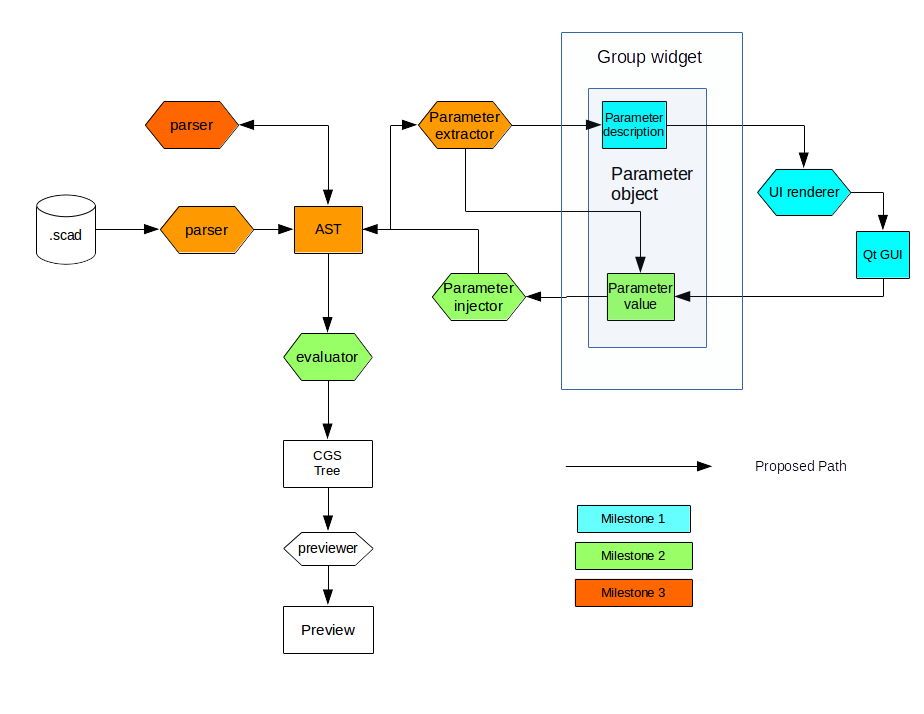
\includegraphics[scale=0.6]{images/flowchart.png}
\caption{Flowchart of Customizer}
\label{fig:FD1}
\end{figure}
